Yes, it has been somewhat of a hobby trying to break DALL-E. I keep
trying to come up with complicated prompts to create improper results.
What do I consider an improper result? That would be something like a
hand having six fingers, a person having more limbs than they're
supposed to, and more. DALL-E seems to have more trouble making pictures
of women rather than men. Does the model's source material bias towards
pictures of cartoon witches?

The prompt, generated in collaboration with LLaVa, states:

\begin{quote}
\emph{A group of tall, very fit, and proud Native American women from a
collegiate volleyball team confidently stride across the campus green.
Their towering stature - each woman measures at least 200 cm - is
evident in their very well-built muscular physiques developed through
frequent training sessions in university gyms. Their away game uniforms
distinguish them from the majority of students who are shorter and less
active, making it clear that they stand out among their peers.}
\end{quote}

The picture:

\begin{figure}
\centering
\pandocbounded{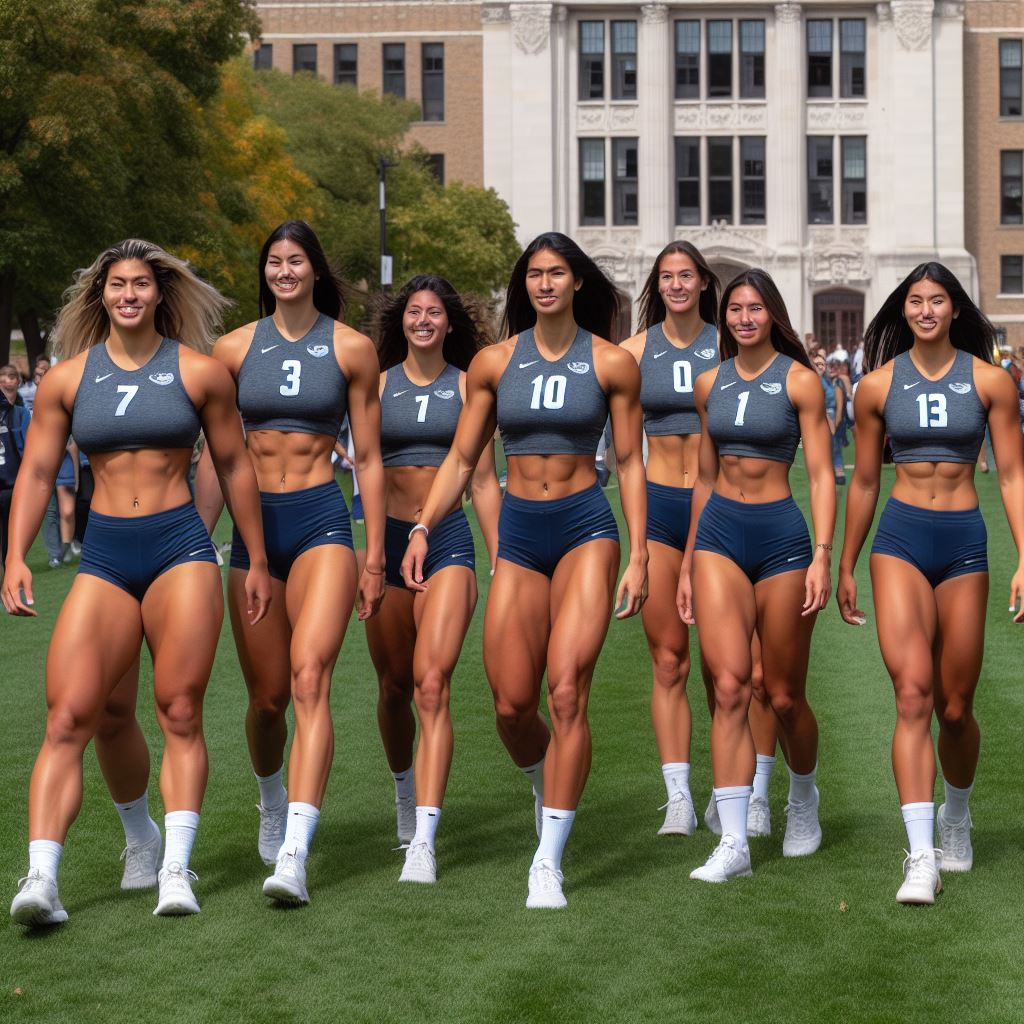
\includegraphics[keepaspectratio]{\%7B\%7Bsite.url\%7D\%7D/img/threelegsagain.jpg}}
\caption{``A group of tall, very fit, and proud Native American women
from a collegiate volleyball team confidently stride across the campus
green. Their towering stature - each woman measures at least 200 cm - is
evident in their very well-built muscular physiques developed through
frequent training sessions in university gyms. Their away game uniforms
distinguish them from the majority of students who are shorter and less
active, making it clear that they stand out among their peers.''}
\end{figure}

One of them clearly has three legs! One of them does not clearly have
three legs but seems to. This is an example of what the prompt
\emph{should have generated}:

\begin{figure}
\centering
\pandocbounded{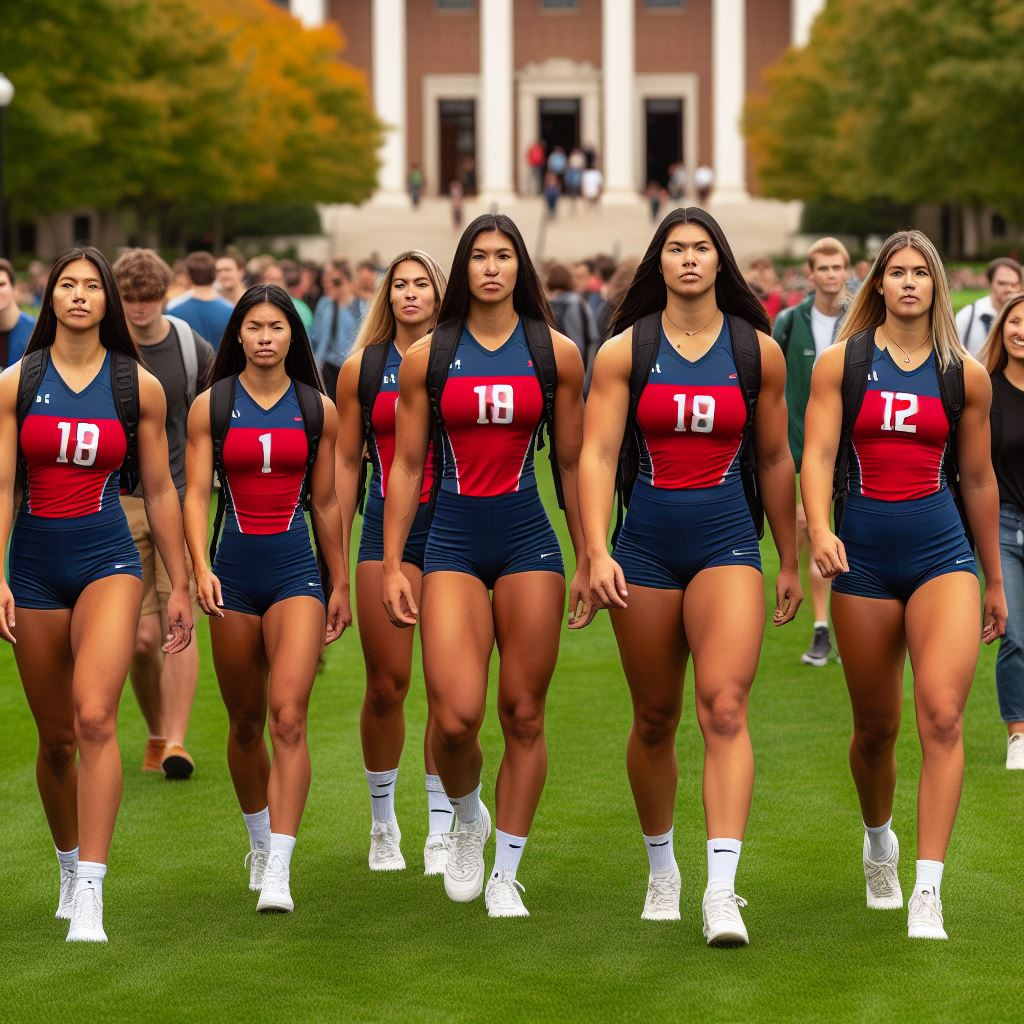
\includegraphics[keepaspectratio]{\%7B\%7Bsite.url\%7D\%7D/img/schooldays.jpg}}
\caption{``A group of tall, very fit, and proud Native American women
from a collegiate volleyball team confidently stride across the campus
green. Their towering stature - each woman measures at least 200 cm - is
evident in their very well-built muscular physiques developed through
frequent training sessions in university gyms. Their away game uniforms
distinguish them from the majority of students who are shorter and less
active, making it clear that they stand out among their peers.''}
\end{figure}

This is another example of what should have happened:

\begin{figure}
\centering
\pandocbounded{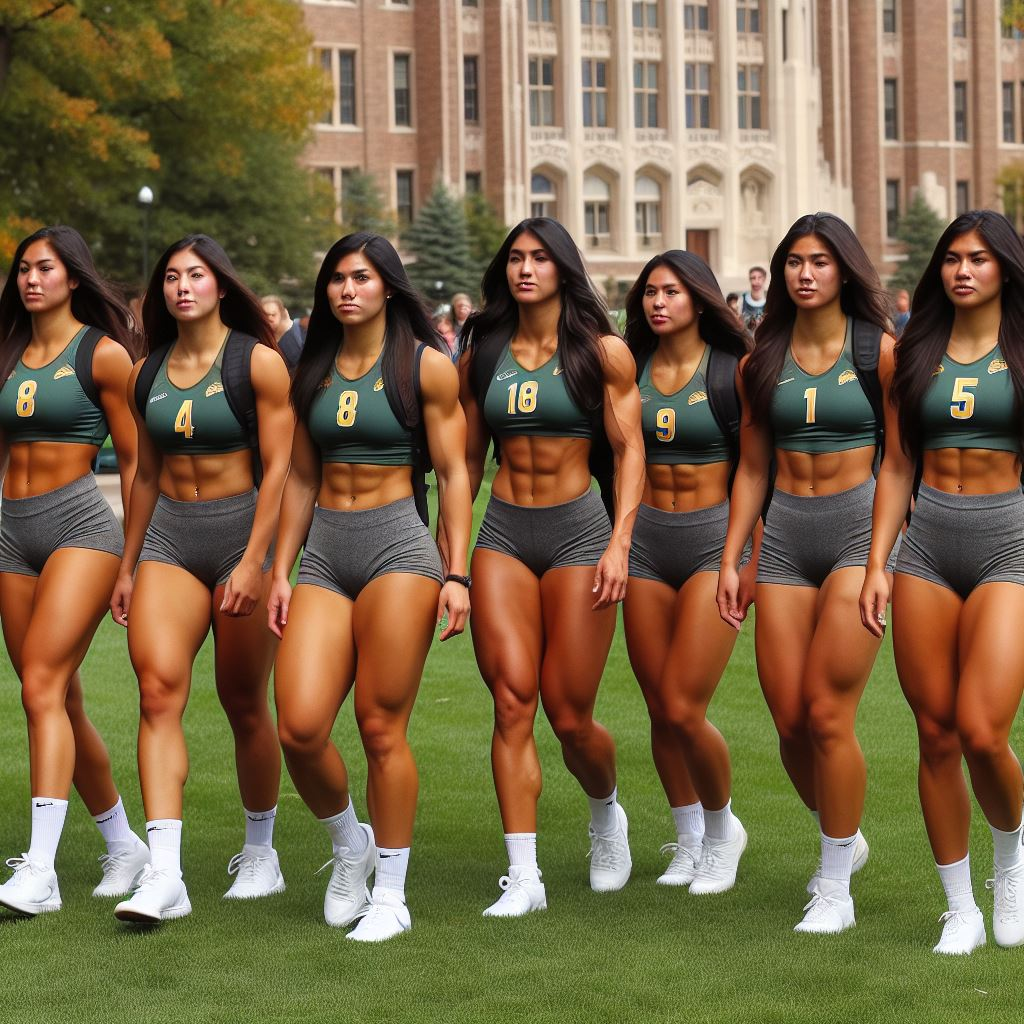
\includegraphics[keepaspectratio]{\%7B\%7Bsite.url\%7D\%7D/img/schooldays2.jpg}}
\caption{``A group of tall, very fit, and proud Native American women
from a collegiate volleyball team confidently stride across the campus
green. Their towering stature - each woman measures at least 200 cm - is
evident in their very well-built muscular physiques developed through
frequent training sessions in university gyms. Their away game uniforms
distinguish them from the majority of students who are shorter and less
active, making it clear that they stand out among their peers.''}
\end{figure}

There is a list of
\href{https://en.wikipedia.org/w/index.php?title=List_of_horror_films_set_in_academic_institutions&oldid=1203533874}{movies
that are horror stories set at colleges/universities} that the first
picture would be appropriate to use with. As to the other two? Well,
there is a
\href{https://en.wikipedia.org/wiki/Category:Films_set_in_universities_and_colleges}{massive
category on Wikipedia for films in that area}.

For spitballing ideas, image generators may be useful in some instances
I suppose. You just have to avoid the cases where they
\href{https://en.wikipedia.org/w/index.php?title=Body_horror&oldid=1202000608}{descend
into body horror}.
